\documentclass[11pt]{article}
\usepackage[T1]{fontenc}
\usepackage{lmodern}
\usepackage{amsmath,amssymb,amsthm,mathtools}
\usepackage{microtype}
\usepackage{geometry}
\geometry{letterpaper,margin=.9in}
\usepackage{tikz}
\usetikzlibrary{arrows.meta,calc}
\usepackage{hyperref}
\hypersetup{pdfauthor={Peyton Wang and Daniel Wang},colorlinks=true,linkcolor=black,citecolor=black,urlcolor=blue!45!black}
\usepackage{enumitem}
\setlist[itemize]{nosep,leftmargin=1.5em}
\setlength{\parindent}{0pt}
\setlength{\parskip}{3pt plus 1pt minus 1pt}
\allowdisplaybreaks
\definecolor{piecezero}{HTML}{F2E8D8}
\definecolor{pieceone}{HTML}{DCEAF2}
\definecolor{piecetwo}{HTML}{DDEDE5}
\definecolor{outline}{HTML}{233847}
\definecolor{seam}{HTML}{C78143}
\definecolor{markcolor}{HTML}{B84442}
\newtheorem{theorem}{Theorem}
\newtheorem{lemma}{Lemma}
\newtheorem{proposition}{Proposition}
\theoremstyle{remark}
\newtheorem{remark}{Remark}
\newcommand{\interior}{\operatorname{int}}
\newcommand{\corners}{\operatorname{Vert}}
\newcommand{\pathQ}{\gamma}

\title{A Simple Orthogonal 22-Gon with\\Exactly One Non-Illuminating Pair}
\author{Peyton Wang\\\small Francis Parker High School \and Daniel Wang\\\small Citizen Health}
\date{Working draft v0.7 --- 10 November 2026\\\small Not submitted or peer reviewed}

\begin{document}
\maketitle
\vspace{-1.2em}
\begin{abstract}
We classify all unordered pairs of distinct real interior points in an explicitly specified strictly simple orthogonal 22-gon: exactly one pair, $\{(0,0),(2,2)\}$, does not illuminate. The room consists of three reflected copies of a five-square staircase, with no interior mirror partitions or boundary self-contacts. A lattice-parity obstruction proves darkness after folding onto the staircase. Four smooth seam endpoints fold to convex corners; their reflected continuations reverse and retrace, so they do not evade the obstruction. To illuminate every other pair, we use two rational cylinder decompositions of the four-copy translation unfolding. Explicit finite permutation certificates and an elementary integrality calculation confine dark endpoints to the room's two interior lattice points. The complete reduced cycle lists are printed in the paper.
\end{abstract}

\section{Introduction}
In the polygonal illumination problem, light rays travel in straight lines and reflect specularly from the sides of a polygonal room. A ray that reaches a vertex is terminated. Two interior points are said to \emph{illuminate each other} if some finite trajectory with these reflection rules connects them.

Our goal is the exact classification of distinct interior pairs in this particular room. The darkness argument uses the unfolding obstruction underlying Tokarsky's constructions \cite{Tokarsky1995}; Wolecki gives a related triangle return-path lemma in \cite[Lemma~3.1]{Wolecki2024}. We give the staircase parity argument explicitly and account for its smooth seam endpoints. General finiteness results for rational polygons appear in \cite[Theorem~1.2]{Wolecki2024}.

Illumination and finite blocking on translation surfaces are studied by Hubert--Schmoll--Troubetzkoy \cite{HST} and Leli\`evre--Monteil--Weiss \cite{LMW}. Our four-copy unfolding is square tiled and is a translation cover of the flat torus. The proof below uses explicit cylinder certificates on that unfolding, with every actual polygon vertex marked as forbidden, including the metrically regular convex-vertex lifts.

``Strictly simple'' means that the boundary is a Jordan polygonal curve: it has no repeated vertices, crossed edges, or self-contacts. Only the exterior boundary reflects light; the dashed segments in the construction are open passages, not mirrors. Sections 2--5 give an elementary proof of darkness. Section 6 proves illumination for every other pair, using a four-copy translation unfolding defined there.

Wolecki's 22-sided example \cite[Figure~1]{Wolecki2024} has diagonal walls and, as drawn, a boundary self-contact at one vertex. The room studied here is orthogonal and strictly simple. We determine its complete non-illumination relation among distinct interior points.

\begin{theorem}[Main result]\label{thm:main}
The polygon $Q$ constructed below is strictly simple and orthogonal, with exactly 22 maximal sides and no holes or interior mirror partitions. Among all unordered pairs of distinct points in $\interior(Q)$, its only non-illuminating pair is $\{(0,0),(2,2)\}$.
\end{theorem}

\section{The construction}
Let $P$ be the union of five closed unit squares with lower-left corners
\begin{equation}\label{eq:squares}
(-1,-1),\quad(0,-1),\quad(0,-2),\quad(1,-2),\quad(1,-3).
\end{equation}
Mark two smooth points of its boundary,
\begin{equation}\label{eq:ab}
a=(0,0),\qquad b=(2,-2).
\end{equation}
Take the following isometric copies of $P$:
\begin{equation}\label{eq:copies}
P_0=P,\qquad P_1=\{(x,-y):(x,y)\in P\},\qquad
P_2=\{(4-x,-y):(x,y)\in P\}.
\end{equation}
Their interiors are pairwise disjoint. The first two meet exactly along
\(H=[-1,1]\times\{0\}\), and the latter two meet exactly along
\(V=\{2\}\times[1,3]\). There are no further contacts. Set
\[
Q=P_0\cup P_1\cup P_2,\qquad S=(0,0),\quad T=(2,2).
\]
Both $S$ and $T$ are midpoints of \emph{open passages} between copies and consequently are interior points of $Q$.

\begin{figure}[htbp]
\centering
\begin{minipage}{.34\textwidth}
\centering
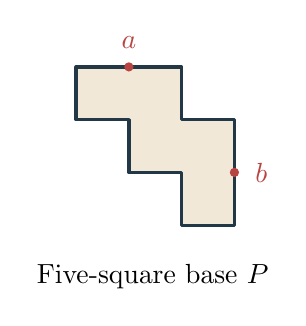
\begin{tikzpicture}[scale=.67,line cap=round,line join=round]
  \fill[piecezero] (-1,-1)--(-1,0)--(1,0)--(1,-1)--(2,-1)--(2,-3)--(1,-3)--(1,-2)--(0,-2)--(0,-1)--cycle;
  \draw[outline,very thick] (-1,-1)--(-1,0)--(1,0)--(1,-1)--(2,-1)--(2,-3)--(1,-3)--(1,-2)--(0,-2)--(0,-1)--cycle;
  \fill[markcolor] (0,0) circle (2.5pt) node[above=3pt] {$a$};
  \fill[markcolor] (2,-2) circle (2.5pt) node[right=4pt] {$b$};
  \node[align=center,below] at (.45,-3.55) {Five-square base $P$};
\end{tikzpicture}
\end{minipage}\hfill
\begin{minipage}{.62\textwidth}
\centering
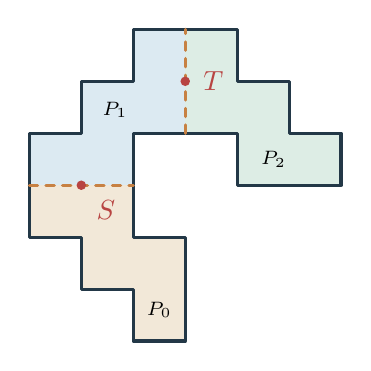
\begin{tikzpicture}[scale=.66,line cap=round,line join=round]
  \fill[piecezero] (-1,-1)--(-1,0)--(1,0)--(1,-1)--(2,-1)--(2,-3)--(1,-3)--(1,-2)--(0,-2)--(0,-1)--cycle;
  \fill[pieceone] (-1,1)--(-1,0)--(1,0)--(1,1)--(2,1)--(2,3)--(1,3)--(1,2)--(0,2)--(0,1)--cycle;
  \fill[piecetwo] (2,3)--(3,3)--(3,2)--(4,2)--(4,1)--(5,1)--(5,0)--(3,0)--(3,1)--(2,1)--cycle;
  \draw[outline,very thick] (-1,-1)--(0,-1)--(0,-2)--(1,-2)--(1,-3)--(2,-3)--(2,-1)--(1,-1)--(1,1)--(3,1)--(3,0)--(5,0)--(5,1)--(4,1)--(4,2)--(3,2)--(3,3)--(1,3)--(1,2)--(0,2)--(0,1)--(-1,1)--cycle;
  \draw[seam,dashed,line width=1.15pt] (-1,0)--(1,0) (2,1)--(2,3);
  \fill[markcolor] (0,0) circle (2.6pt) node[below right=2pt] {$S$};
  \fill[markcolor] (2,2) circle (2.6pt) node[right=3pt] {$T$};
  \node at (1.5,-2.4) {\scriptsize $P_0$};
  \node at (.65,1.45) {\scriptsize $P_1$};
  \node at (3.7,.5) {\scriptsize $P_2$};
\end{tikzpicture}
\end{minipage}
\caption{The five-square base $P$ and the 22-sided room $Q$. The bold exterior outline is reflective. The dashed segments are open seams, not partitions. The two marked points $S$ and $T$ lie in the interior of $Q$.}\label{fig:construction}
\end{figure}

For reproducibility, the counterclockwise sequence of all 22 vertices of $Q$ is
\begin{equation}\label{eq:vertices}
\begin{gathered}
(-1,-1), (0,-1), (0,-2), (1,-2), (1,-3), (2,-3),\\
(2,-1), (1,-1), (1,1), (3,1), (3,0), (5,0),\\
(5,1), (4,1), (4,2), (3,2), (3,3), (1,3),\\
(1,2), (0,2), (0,1), (-1,1).
\end{gathered}
\end{equation}
Every successive edge is horizontal or vertical and nonzero, with successive edges meeting at right angles. The union description (or a direct check of the vertex cycle) shows that the boundary does not self-intersect or self-touch. There are 13 convex vertices and nine reflex vertices, and the area is 15.

The \emph{folding map} $f:Q\to P$ is defined copywise by
\begin{equation}\label{eq:fold}
f|_{P_0}(x,y)=(x,y),\qquad
f|_{P_1}(x,y)=(x,-y),\qquad
f|_{P_2}(x,y)=(4-x,-y).
\end{equation}
These formulas agree on the seams, so $f$ is well defined and continuous. In particular, $f(S)=a$ and $f(T)=b$. The complete preimages of the base marks are
\[
 f^{-1}(a)=\{S,(4,0)\},\qquad f^{-1}(b)=\{(2,-2),T\}.
\]
Visits to a base mark are therefore counted after folding, even when the physical trajectory reaches another preimage.

\section{The lattice obstruction on the staircase}
The next lemma concerns \emph{ordinary} billiard motion in $P$, reflecting only at smooth boundary points and never touching a vertex. Paths have finitely many nonzero straight legs. At each intermediate smooth-wall contact the incoming and outgoing legs satisfy the specular reflection rule.

\begin{lemma}[Parity obstruction]\label{lem:parity}
There is no finite corner-avoiding billiard path in $P$ from $a=(0,0)$ to $b=(2,-2)$.
\end{lemma}
\begin{proof}
First inspect the integer points in $P$. There are no interior integer points. Its only integer boundary points that are not vertices are $a$ and $b$. More explicitly, its seven convex corners are
\[
(-1,-1),\ (-1,0),\ (0,-2),\ (1,-3),\ (1,0),\ (2,-3),\ (2,-1),
\]
and its three reflex corners are
\[
(0,-1),\ (1,-2),\ (1,-1).
\]

Suppose an ordinary billiard path from $a$ to $b$ exists. Unfold its finitely many reflections, reflecting the staircase instead of bending the path. The result is a single straight segment starting at $a=(0,0)$ and ending at an image $B$ of $b$. Reflection across any wall $x=c$ or $y=d$, where $c,d\in\mathbb{Z}$, preserves both coordinate parities. Since $b$ has even coordinates, $B\in(2\mathbb{Z})^2$. Further, $B\ne(0,0)$ because unfolding preserves the positive length of the path.

Write $B=2^r z$, where $r\ge 1$ and $z\in\mathbb{Z}^2$ has at least one odd coordinate; choose $r$ maximal. Then $z$ is a lattice point strictly between $0$ and $B$ on the unfolded segment. Fold $z$ back to $P$ along the proposed itinerary. All inverse unfolding maps are compositions of reflections in integer-coordinate lines and therefore preserve integrality and coordinate parities. The image of $z$ lies on the original path and is an integer point of $P$ with an odd coordinate. It is neither $a$ nor $b$, hence must be a vertex of $P$. This would make the original path hit a vertex, a contradiction.
\end{proof}

\begin{remark}
The lemma is valid for arbitrary finite path length, direction, and number of reflections. The obstruction arises from the parity of an \emph{unfolded endpoint}, not from a bounded search over directions.
\end{remark}

\section{What happens at the seams?}
A billiard trajectory in $Q$ need not fold into an ordinary billiard trajectory in $P$ at every instant. The exceptions are precisely the smooth boundary points of $Q$ lying at the ends of open seams. It is important to account for them rather than treating them as forbidden corners of $Q$.

Away from the seams, each branch of $f$ is an isometry. A reflection at a smooth exterior wall of $Q$ thus becomes an ordinary reflection at a smooth wall of $P$, unless that point is a seam endpoint. A straight passage across the \emph{interior} of either seam also becomes an ordinary reflection in $P$: the adjacent folding maps agree at the seam and reverse the normal component of velocity.

The four seam endpoints are
\begin{equation}\label{eq:exceptional}
E_1=(-1,0),\qquad E_2=(1,0),\qquad
E_3=(2,1),\qquad E_4=(2,3).
\end{equation}
Each $E_j$ is smooth on the external boundary of $Q$, yet folds to a convex right-angle corner of $P$:
\[
\begin{array}{c|c|c}
\text{smooth point of }Q & \text{vertex of }P & \text{exterior mirror in }Q\\ \hline
(-1,0) & (-1,0) & \text{vertical}\\
(1,0) & (1,0) & \text{vertical}\\
(2,1) & (2,-1) & \text{horizontal}\\
(2,3) & (2,-3) & \text{horizontal}
\end{array}
\]

\begin{lemma}[Seam-endpoint reversal]\label{lem:reversal}
If a corner-avoiding billiard trajectory in $Q$ reflects at a seam endpoint $E_j$, its folded trajectory in $P$ instantaneously \emph{reverses its entire velocity} at the corresponding convex corner and retraces its incoming route.
\end{lemma}
\begin{proof}
For example, consider $E_2=(1,0)$. A ray approaching from $P_1$ with physical velocity $(u,-v)$ ($u,v>0$) folds via $(x,y)\mapsto(x,-y)$ to incoming velocity $(u,v)$ in $P$. At $E_2$, the actual exterior mirror is vertical, so the physical outgoing velocity becomes $(-u,-v)$ and the ray travels into $P_0$. Folding this outgoing segment by the identity gives $(-u,-v)$, the negative of the incoming folded velocity. Reversing the time orientation gives the same conclusion for arrivals from $P_0$.

At $E_1$ the same two reflections occur in the opposite horizontal direction. At $E_3$ and $E_4$, interchange the horizontal and vertical coordinates: the physical exterior reflection negates the vertical component, while switching copies across the vertical seam negates the horizontal component. In every case, the combined effect is $(\alpha,\beta)\mapsto(-\alpha,-\beta)$.
\end{proof}

\begin{figure}[htbp]
\centering
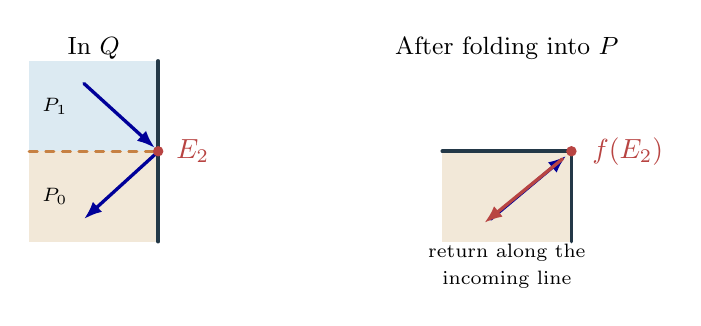
\begin{tikzpicture}[>=Latex,scale=.82,line cap=round]
  \begin{scope}
    \fill[pieceone] (-1,0) rectangle (1,1.4);
    \fill[piecezero] (-1,-1.4) rectangle (1,0);
    \draw[outline,line width=1.3pt] (1,-1.4)--(1,1.4);
    \draw[seam,dashed,line width=1pt] (-1,0)--(1,0);
    \draw[blue!60!black,very thick,-{Latex[length=2.3mm]}] (-.15,1.05)--(.95,.05);
    \draw[blue!60!black,very thick,-{Latex[length=2.3mm]}] (.95,-.05)--(-.15,-1.05);
    \fill[markcolor] (1,0) circle(2.3pt) node[right=3pt] {$E_2$};
    \node at (0,1.6) {\small In $Q$};
    \node at (-.6,.7) {\scriptsize $P_1$};
    \node at (-.6,-.7) {\scriptsize $P_0$};
  \end{scope}
  \begin{scope}[xshift=6.4cm]
    \fill[piecezero] (-1,-1.4) rectangle (1,0);
    \draw[outline,line width=1.3pt] (-1,0)--(1,0)--(1,-1.4);
    \draw[blue!60!black,very thick,-{Latex[length=2.3mm]}] (-.25,-1.05)--(.92,-.07);
    \draw[markcolor,very thick,-{Latex[length=2.3mm]}] (.86,-.12)--(-.35,-1.11);
    \fill[markcolor] (1,0) circle(2.3pt) node[right=4pt] {$f(E_2)$};
    \node at (0,1.6) {\small After folding into $P$};
    \node[align=center] at (0,-1.78) {\scriptsize return along the\\[-2pt]\scriptsize incoming line};
  \end{scope}
\end{tikzpicture}
\caption{The exceptional event at the horizontal seam endpoint $E_2$. A normal mirror reflection in $Q$ switches copies and becomes an exact retracing at a convex vertex of $P$. The diagrams show local geometry, not a possible complete connecting path.}\label{fig:reverse}
\end{figure}

Every original corner of $P$ gives one corner incidence in each of $P_0,P_1,P_2$. Of these 30 incidences, two meet at each of the four smooth endpoints $E_j$ (eight incidences total). All remaining 22 incidences are actual vertices of $Q$. In particular, \emph{no reflex corner of $P$ is the image of a smooth point of $Q$}. It follows that a valid $Q$-trajectory can fold only to ordinary billiard motion in $P$, occasionally interrupted by the corner reversals of Lemma~\ref{lem:reversal}.

\section{Why reversals do not create a connecting path}
\begin{lemma}[Reversals do not help]\label{lem:nohelp}
There is no finite path from $a$ to $b$ in $P$ obtained by ordinary billiard reflections at smooth walls together with the additional rule that a path may reverse its velocity and retrace itself at a convex corner. Reflex corners remain forbidden.
\end{lemma}
\begin{proof}
Suppose such a path exists. Stop it at its first arrival at $b$, and retain only the subpath beginning at its \emph{last} visit to $a$ before that arrival. The resulting path $\gamma$ starts at $a$, ends at $b$, and contains no interior occurrence of either marked point. There are finitely many such visits because the path has finitely many nonzero straight legs. This truncation takes place in $P$: a visit to $a$ counts regardless of which preimage of $a$ the original path visits in $Q$.

Assume $\gamma$ has a corner reversal, and choose the first one. Up to that event, motion consists entirely of ordinary billiard reflections. Ordinary billiard motion is deterministic and reversible. Once the first reversal takes place, the path must retrace the entire preceding route in reverse order, ultimately reaching $a$. It cannot reach $b$ during this retracing, since the corresponding point would already have occurred before the reversal, contradicting the first-arrival choice of $b$. Thus the path revisits $a$ before reaching $b$, contradicting the last-visit choice of $a$.

Hence $\gamma$ has no reversals and is an ordinary corner-avoiding billiard path from $a$ to $b$, contrary to Lemma~\ref{lem:parity}.
\end{proof}

\begin{proof}[Proof of the darkness assertion in Theorem~\ref{thm:main}]
The explicit construction and boundary cycle establish that $Q$ is a strictly simple orthogonal polygon with 22 maximal sides, no holes, and $S,T\in\interior(Q)$.

Suppose a finite billiard trajectory joins $S$ to $T$ in $Q$. It cannot be axis-parallel: reflecting in a horizontal or vertical wall preserves the property that one velocity component vanishes, whereas $S$ and $T$ differ in both coordinates. Consequently every straight leg meets either seam transversely, if at all. Since the trajectory has finitely many legs and each leg crosses each seam at most once, its folding by $f$ splits into finitely many straight segments and events.

By the seam analysis, the image is a finite path from $a=f(S)$ to $b=f(T)$ following the rules of Lemma~\ref{lem:nohelp}. That lemma forbids such a path. Therefore no finite corner-avoiding billiard trajectory joins $S$ and $T$.
\end{proof}


\section{Every other interior pair is illuminated}\label{sec:cylinders}
Here and throughout, a pair means two \emph{distinct} interior points. Self-return trajectories and boundary sources are not part of the classification.

\subsection{The four-copy unfolding}
Form a translation surface $M$ from four copies of $Q$, labelled by
$\varepsilon=(\varepsilon_1,\varepsilon_2)\in\{1,-1\}^2$.
In the copy labelled $\varepsilon$, use developing coordinates
$(\varepsilon_1x,\varepsilon_2y)$, up to integer translations.
Across a vertical exterior wall, glue to the copy with the first sign reversed;
across a horizontal exterior wall, reverse the second sign. Internal unit-cell
edges are ordinary translation identifications on the same sheet.
The resulting surface consists of 60 unit squares. Let $\Sigma$ be the set
of all lifts of actual polygon vertices. Include convex vertices in $\Sigma$
even though their lifts have total angle $2\pi$.
Smooth boundary lattice points and interior lattice points are not in $\Sigma$.
A straight geodesic avoiding $\Sigma$ projects to a legal billiard trajectory.

The map $\tau$ that replaces $\varepsilon$ by $-\varepsilon$ is an isometry
with derivative $-I$, and projects to the same point of $Q$.
It has no fixed point outside $\Sigma$: an interior point has four distinct
lifts, while a smooth wall point identifies only one of the two sign changes.
Only at polygon vertices can the two simultaneous sign changes be identified.

A \emph{regular cylinder} in a rational direction is a maximal open annulus
of parallel closed geodesics avoiding $\Sigma$. In coordinates it is
$(\mathbb R/L\mathbb Z)\times(0,h)$; its closure is the image of a closed strip.
The involution $\tau$ cannot preserve a regular cylinder. Indeed, on such a
cylinder it would have the form $(u,v)\mapsto(c-u,h-v)$, which has two fixed
points at $v=h/2$, contrary to the preceding observation.

\begin{lemma}[Two-cylinder visibility]\label{lem:cylinder}
Suppose a rational direction decomposes $M$ into two regular cylinders,
exchanged by $\tau$, whose closures cover $M$.
If an interior point $A$ has a lift in one of the open cylinders,
then $A$ illuminates every other interior point $B$ of $Q$.
\end{lemma}
\begin{proof}
Let $\widehat A$ lie in the open cylinder $C$. Choose a lift $\widehat B$;
replace it by $\tau\widehat B$ if necessary so that it lies in $\overline C$.
Since $A\ne B$, their lifts are distinct. Represent them in a closed
covering strip $\mathbb R\times[0,h]$ as $(u_A,v_A)$ and $(u_B,v_B)$,
where $0<v_A<h$ and $0\le v_B\le h$. For $0<t<1$, the interpolated
height $(1-t)v_A+tv_B$ lies strictly between $0$ and $h$. Thus the entire
open segment between the representatives lies inside the open strip.
Its image avoids $\Sigma$ in its interior; the endpoint also avoids $\Sigma$
because $B$ is interior to $Q$. Projection to $Q$ gives a finite legal
billiard path. Compactness of the segment and its avoidance of the finite
marked set ensure that only finitely many wall crossings occur.
\end{proof}

\begin{figure}[htbp]
\centering
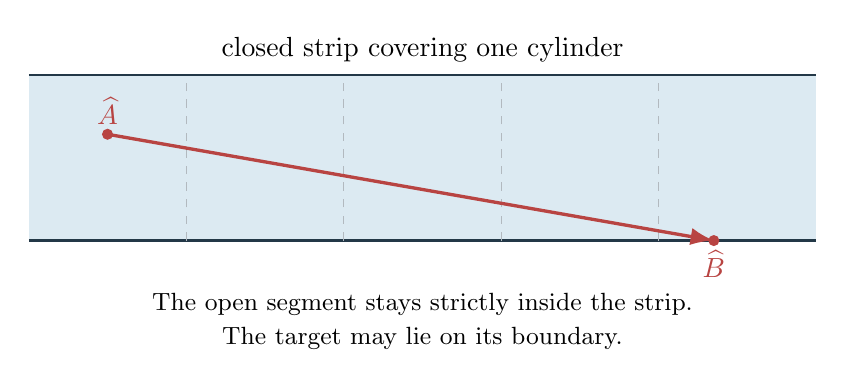
\begin{tikzpicture}[x=1cm,y=1cm,>=Latex]
\fill[pieceone] (0,0) rectangle (10,2.1);
\draw[outline,thick] (0,0)--(10,0) (0,2.1)--(10,2.1);
\foreach \x in {2,4,6,8} {\draw[outline!35,dashed] (\x,0)--(\x,2.1);}
\fill[markcolor] (1,1.35) circle(2pt) node[above] {$\widehat A$};
\fill[markcolor] (8.7,0) circle(2pt) node[below] {$\widehat B$};
\draw[markcolor,very thick,-{Latex}] (1,1.35)--(8.7,0);
\node[above] at (5,2.15) {closed strip covering one cylinder};
\node[below,align=center] at (5,-.55) {\small The open segment stays strictly inside the strip.\\
\small The target may lie on its boundary.};
\end{tikzpicture}
\caption{The visibility step, shown schematically in a cylinder's covering strip.
Dashed lines indicate repeated periods, not mirrors. No assertion is made
that the connecting segment follows the cylinder's periodic direction.}
\label{fig:strip}
\end{figure}

\subsection{Two finite cylinder certificates}\label{sec:certificate}
For this room, the directions $(p,q)=(4,7)$ and $(7,4)$ satisfy the hypothesis
of Lemma~\ref{lem:cylinder}. They were found by a finite scan of primitive integer directions; the strip permutation below certifies the two selected inputs. The proof needs only the two displayed certificates, not completeness of that scan.

The reason for using two directions is arithmetic. In one direction, a dark endpoint must satisfy $qx-py,qx+py\in\mathbb Z$, which implies $2qx,2py\in\mathbb Z$ but can leave nonintegral candidates. The two chosen directions together force $(x,y)\in\mathbb Z^2$, as shown in Section~\ref{sec:eliminate}. Here is an explicit finite prescription for checking the two cylinder inputs.

Let $\mathcal C$ be the 15 cell lower-left corners determined by
\eqref{eq:squares}--\eqref{eq:copies}. In lexicographic order they are
\[
\begin{gathered}
(-1,-1),\ (-1,0),\ (0,-2),\ (0,-1),\ (0,0),\ (0,1),\\
(1,-3),\ (1,-2),\ (1,1),\ (1,2),\ (2,1),\ (2,2),\\
(3,0),\ (3,1),\ (4,0).
\end{gathered}
\]
Reflection across $y=0$ sends the unit cell with lower-left corner $(m,n)$
to the cell with lower-left corner $(m,-n-1)$; reflecting a cell is not the
same as reflecting its lower-left corner.
Order the 60 squares of $M$ lexicographically by cell, then by sheet in the order
$(+,+),(-,+),(+,-),(-,-)$, numbering from 0.
Because $Q$ is the union of its cells with no internal mirrors, a shared
unit edge is an open passage between the adjacent cells.
The right-neighbour permutation $r$ sends square $((m,n),(\varepsilon_1,\varepsilon_2))$ to
$((m+\varepsilon_1,n),(\varepsilon_1,\varepsilon_2))$ when that cell is in $\mathcal C$, and otherwise to
$((m,n),(-\varepsilon_1,\varepsilon_2))$. Similarly the up-neighbour permutation $u$ moves to
$((m,n+\varepsilon_2),(\varepsilon_1,\varepsilon_2))$ when possible, and otherwise to
$((m,n),(\varepsilon_1,-\varepsilon_2))$.

In each square divide its bottom edge into $q$ open intervals
$(j/q,(j+1)/q)$, $0\le j<q$. Following direction $(p,q)$ from one bottom
crossing to the next induces the permutation
\[
 (i,j)\longmapsto
 \left(u\left(r^{\lfloor(j+p)/q\rfloor}(i)\right),\ (j+p)\bmod q\right).
\]
The permutation preserves the within-interval offset $t-j/q$, so each cycle closes every leaf in its open interval. A cycle therefore describes an open annular strip of regular leaves. These strips
cover every leaf whose transverse coordinate $qx-py$ is nonintegral.
All marked points have integral developing coordinates, so none lies
inside such a strip. The complete cycle lists are included in
\texttt{certificate.json}, and the standalone standard-library Python program
\texttt{verify\_cylinders.py} regenerates them from the cell formulas.
The results are
\[
\begin{array}{c|r|c|c}
(p,q)&\text{slots}&\text{cycle lengths}&\text{number of cycles}\\\hline
(4,7)&420&210,210&2\\
(7,4)&240&120,120&2
\end{array}
\]
The strips need not initially be maximal relative to $\Sigma$.
Every regular cylinder contains one of these strips: the complement of the
integral transverse levels is dense. Thus there are at most two regular
cylinders. There are at least two, since $\tau$ cannot preserve a cylinder.
Consequently there are exactly two, exchanged by $\tau$; their closures cover
$M$, again by density. This proves the required cylinder input from the
finite permutations.

\paragraph{A compact printed certificate.}
Write $T$ for the slot permutation above. Since $\gcd(p,q)=1$, the residue
$j$ visits every value modulo $q$ and first returns to $0$ after exactly
$q$ steps. Hence the first-return permutation
$\Phi_{p,q}(i)=\pi_1(T^q(i,0))$ acts on just the 60 squares.
Each cycle of length $n$ for $\Phi_{p,q}$ corresponds to a cycle of length
$nq$ for $T$, and every cycle of $T$ occurs this way.
The successive exponents of $r$ are $(0,1,0,1,0,1,1)$ for $(4,7)$ and
$(1,2,2,2)$ for $(7,4)$. Thus, with composition read from right to left,
\[
\Phi_{4,7}=(ur)^2u(ur)u(ur)u,
\qquad
\Phi_{7,4}=(ur^2)^3(ur).
\]
Using the square numbering specified above, their complete cycle
decompositions are listed below. Each parenthesis denotes one closed cycle;
line breaks within a parenthesis only save space.
\[
\small
\begin{array}{c|l}
(p,q)&\text{cycles of }\Phi_{p,q}\\ \hline
(4,7)&\begin{gathered}
(0,43,47,54,52,48,41,4,13,36,59,34,38,23,11,\\
15,32,57,19,26,6,28,24,9,21,17,30,2,50,45),\\[2pt]
(1,27,31,29,10,5,46,49,18,22,7,44,40,42,53,\\
3,25,16,51,55,58,37,33,35,20,56,39,14,12,8)
\end{gathered}\\[7pt]
(7,4)&\begin{gathered}
(0,1,47,10,13,39,52,40,32,51,59,58,38,53,19,\\
25,21,33,41,18,6,7,24,20,50,46,11,31,30,12),\\[2pt]
(2,29,36,3,15,14,28,8,9,44,57,35,26,5,17,\\
16,34,22,23,27,4,42,45,56,48,49,43,55,54,37)
\end{gathered}
\end{array}
\]
The two displayed cycles for each direction cover all 60 squares and give the
cycle lengths in the table. The included checker also regenerates these
reduced permutations and compares them with \texttt{certificate.json}.


\subsection{Eliminating all other sources}\label{sec:eliminate}
Fix one of these directions $(p,q)$. On sheet $(\varepsilon_1,\varepsilon_2)$, the transverse value at a lift of $A=(x,y)$ is
$\varepsilon_1qx-\varepsilon_2py$ modulo integers. Thus the four values are
\[
 \pm(qx-py),\qquad \pm(qx+py).
\]
If either $qx-py$ or $qx+py$ is nonintegral, a lift of $A$ lies in an open strip, hence in an open regular
cylinder: the strips cover the nonintegral transverse levels.
Lemma~\ref{lem:cylinder} then shows that $A$ illuminates every other
interior point. Therefore each endpoint of a dark pair must satisfy
\[
 7x-4y,\ 7x+4y,\ 4x-7y,\ 4x+7y\ \in\mathbb Z.
\]
Adding and subtracting gives $14x,8x,8y,14y\in\mathbb Z$, hence
$2x,2y\in\mathbb Z$. Write $x=k/2$, $y=\ell/2$ with $k,\ell\in\mathbb Z$.
Integrality of $(7k+4\ell)/2$ forces $k$ even; integrality of $(4k+7\ell)/2$
forces $\ell$ even. Thus $(x,y)\in\mathbb Z^2$. Conversely every lattice point
satisfies the four conditions.

The cell construction has only two interior lattice points, $S=(0,0)$ and
$T=(2,2)$. This can be checked directly from the 15 squares: $(x,y)$ is an
interior lattice point exactly when all four cells with lower-left corners
in $\{x-1,x\}\times\{y-1,y\}$ occur. The included program checks this as well.
Every other interior point illuminates every other distinct interior point.
The preceding darkness proof excludes a connection between $S$ and $T$.
This completes the proof of Theorem~\ref{thm:main}.

\section{Scope and reproduction}
The classification covers distinct real interior endpoints in the specified
polygon. It does not classify boundary endpoints or self-return trajectories,
and it gives no lower bound for other polygons.
The darkness argument is analytic; the illumination argument combines the
strip lemma and the integrality calculation with the two finite permutation
certificates. The cell formulas, return-map words and complete reduced cycle
lists printed here suffice to verify those finite inputs without external
files. The JSON certificate and Python checker are supplementary
reproduction tools. Run
\begin{verbatim}
python3 verify_cylinders.py --check
\end{verbatim}
from the manuscript directory to regenerate and compare both certificates.
The program requires only Python 3 and the included JSON file.
The illustrated companion \texttt{explainer.html} shows the strip construction
and the exceptional-source conditions.

\paragraph{Acknowledgements and AI assistance.}
The authors used the AI systems ChatGPT (OpenAI) and Claude (Anthropic) extensively while exploring candidate geometries, developing explanations, and refining the proof. The authors take responsibility for the mathematical content of any eventual submitted version.

\begin{thebibliography}{9}
\bibitem{Tokarsky1995}
G.~W. Tokarsky, ``Polygonal Rooms Not Illuminable from Every Point,''
\emph{The American Mathematical Monthly} \textbf{102} (1995), no.~10, 867--879.
\url{https://doi.org/10.1080/00029890.1995.12004679}.

\bibitem{Wolecki2024}
A.~Wolecki, ``Illumination in Rational Billiards,''
\emph{arXiv:1905.09358v3} (2024), Theorem~1.2, Lemma~3.1 and Figure~1.
\url{https://arxiv.org/abs/1905.09358v3}.

\bibitem{HST}
P.~Hubert, M.~Schmoll and S.~Troubetzkoy,
``Modular Fibers and Illumination Problems,''
\emph{International Mathematics Research Notices} (2008), Article ID rnn011.
\url{https://arxiv.org/abs/math/0602394}.

\bibitem{LMW}
S.~Leli\`evre, T.~Monteil and B.~Weiss,
``Everything is illuminated,''
\emph{Geometry \& Topology} \textbf{20} (2016), 1737--1762.
\url{https://doi.org/10.2140/gt.2016.20.1737}.
\end{thebibliography}
\end{document}
